\documentclass[12pt, git, final]{rureport}


\begin{document} % this tells the compiler that it is time to make
                 % text to print instead of just getting ready.
\maketitle  % make a title page from the Title, Date, and Author

%\fxnote{skoða titil á skýrslu, sbr. forsíðu}

%\section*{Errata} %%section* avoids putting a number 
%
\section{Inngangur} % sections break up the document into pieces
Himingeimurinn er fyrir mörgum jafn áhugaverður og hann er stór, menn hafa öldum saman spáð mikið í himintunglum ásamt öðrum fyrirbærum út í hinum víðamikla geimi frá örófi alda, jafnvel verið orsakavaldur styrjalda. Af því hópurinn deilir sömu hrifningu á himinhvolfinu, var ákveðið að ná í gögn um sólmyrkva jarðar, stríð og átök sem herjað hafa á jörðina ásamt vopnasölu út um heim allan. Fyrst og fremst vildi hópurinn skoða hvernig átök heimsins dreifast niður á jörðina, hversu oft og hvar lenda sólmyrkvarnir á jörðina á hverju ári og hvort það sé möguleiki á fylgni milli fjölda sólmyrkva og fjölda stríðsátaka? Þessir útgangspunktar verða skoðaðir nánar og þeim gefin frekari skil í niðurstöðunum.  
\section{Framkvæmd}
\subsection{Hnötturinn}
Við gerð hnattarins þá var notast við Basemap sem er viðbót við matplotlib. Til að fá hnöttin raunverulegri var notast við bluemarble fall sem er að finna í Pillow \cite{pillow} pakkanum en það tekur myndir frá NASA \cite{bluemarble} og varpar þeim á hnöttinn. Notast var við gögn úr gagnagrunninum til að fá hnit sólmyrkvana frá 1901-2100 og til að framkalla svo snúning jarðarinnar þá voru búnar til 180 myndir á tveggja lengdargráðu fresti, og þeim skeytt saman í hreyfimynd eða myndband eftir henntisemi notanda með MoviePy pakkanum \cite{moviepy}.
 
\subsection{Myndrænt notendaviðmót}



\section{Aðferð}
\subsection{Hönnun}
Við hönnun á GUI þá var notast við Qt4 Designer \cite{qt4}. Ákveðið var að það yrði innskráningar gluggi (sjá mynd \ref{fig:logScreen}). Hann hefur tvo tilganga, annars vegar er hægt að slá inn upplýsingar til að búa til gagnagrunninn ef hann er ekki til staðar í tölvunni með því að ýta á 'Populate DB' hnappinn og hins vegar til að tengjast gagnagrunninum með því að ýta á ok hnappinn. Forritið lætur svo notandan vita hvort tenging hafi tekist( sjá mynd \ref{fig:logsucces}). Eftir það sprettur upp aðal gluggi forritsins(sjá mynd \ref{fig:openScreen}), sem er í grunninn heimskort með tímastiku fyrir neðan það og hægra megin við það eru 4 dálkar sem sína ástand viðkomandi árs, en hann er útskýrður  í kafla \ref{virkni}


\subsection{Gögn}
Fyrst var farið á veraldarvefin og leitað af gögnum sem hægt væri að vinna með, gögnin voru fundin á síðu hjá NASA \cite{Eclipse}, Stockholm international peace research institution \cite{weapon} og Háskólanum í Uppsölum í Svíþjóð \cite{conflict}. Gögnin voru tekin inn á csv formi, þau voru svo hreinsuð í python og unnið með þau sem Dataframes áður en þeim var flutt inn í gagnagrunninn sjálfan. Þegar kom að því að túlka hnitin var stuðst við pygeocoder pakkann \cite{geocoder}


\subsection{Á bakvið tjöldin - undirvirknir forrits}
Þó svo að eitt forrit sé keyrt í command glugganum, þá fer virkjast aragrúi af undirforritum eins og sést á mynd \ref{fig:diagram}. Aðalforritið hefur tvær leiðir til að byrja með, skrá sig inn í gagnagrunn sem er nú þegar fyrir hendi, eða búa hann til. Ef notandi velur að búa til gagnagrunn, keyrir forritið populate\_sql.py sem býr til gagnagrunninn, allar töflurnar og fyllir þær, notandinn þarf þó að vera búinn að fylla út alla dálka á fyrsta spretti glugganum og passa nafnið á nýja gagnagrunninum sé ekki frátekið en ef svo er kemur villumelding.

Þegar notandi er búinn að búa til gagnagrunninn og aðalglugginn opnast er fallið komið inn í GUI.py skránna, sem hefur eiginlega tvískipta virkni, annars vegar að teikna staðseningar inná kort sem eru smellanlegir og að tala við gagnagrunninn, ná í upplýsingar fyrir alla viðeigandi dálka. Ef smellt er á staðsetningu, nær forritið líka í allar viðeigandi upplýsingar og birtir í viðkomandi dálkum.



\subsection{Virkni forrits}\label{virkni}
Eftir að notandi er búinn að tengjast gagnagrunni þá getur hann skoðar ýmsar upplýsingar út frá árum. Það er hægt að hreyfa við stiku til að fá ákveðið ár eða slá inn ártalið til að fá viðkomandi upplýsingar um hvað gerðist á því ári. Upplýsingarnar skila sér svo á kortinu sem er á upphafskjánnum og það birtast upplýsingar í dálkum hægra megin fyrir. 


\section{Niðurstöður}\label{nidurstodur}

Þegar staðsetningar sólmyrkvana er teiknuð á hnöttinn sást að hringir myndast á breiddargráðum 60$^{\circ}$-75$^{\circ}$ bæði á norður- (sjá mynd \ref{fig:3DNP}) og suðurhveli jarðar (sjá mynd \ref{fig:3DSP}) og sú lína spannar ca 43,6\% af öllum sólmyrkvunum sem hafa verið á jörðinni frá tímabilinu 1901 - 2100. Hægt er að sjá að á svæðum sem sólmyrkvarnir mynda þéttan kjarna, því færri stríð hafa geisað á þeim svæðum sbr 60$^{\circ}$-75$^{\circ}$
\pagebreak

\begin{figure}
	\centering
	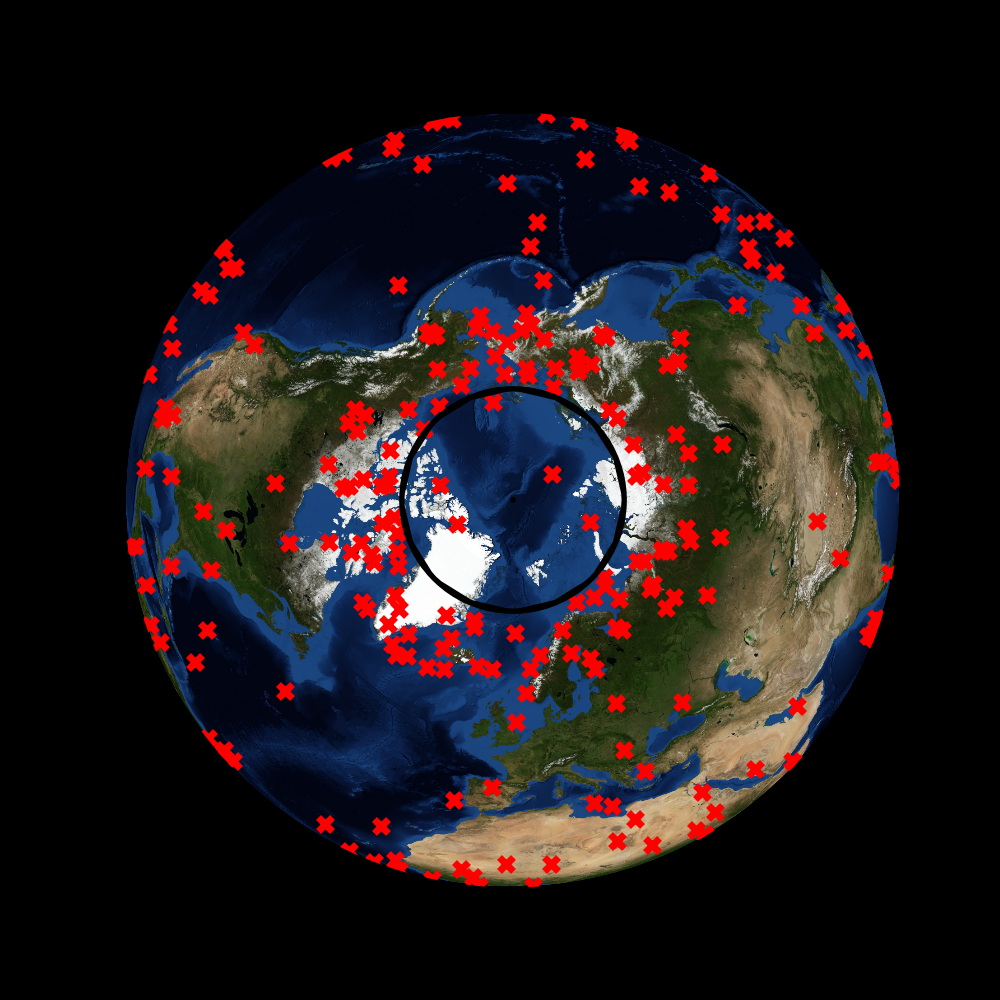
\includegraphics[width=10cm]{3DNP.png}
	\caption{Sólmyrkvarnir séð frá Norður pólnum}
	\label{fig:3DNP}
\end{figure}

\begin{figure}
	\centering
	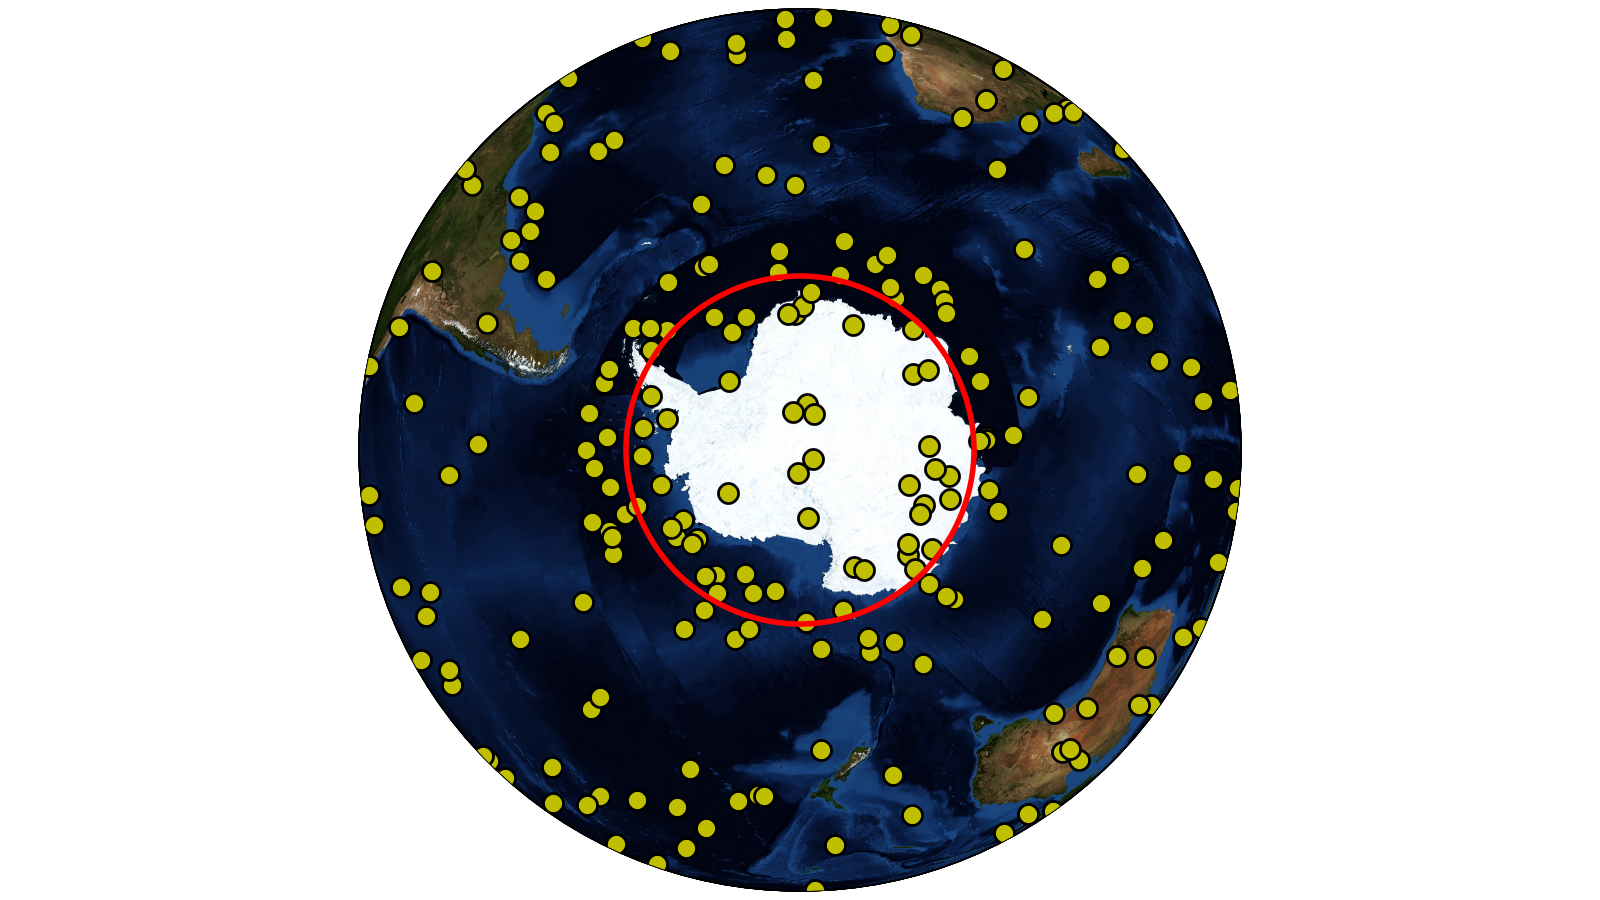
\includegraphics[width=10cm]{3DSP.png}
	\caption{Sólmyrkvarnir séð frá Suður pólnum}
	\label{fig:3DSP}
\end{figure}

\begin{figure}
	\centering 
	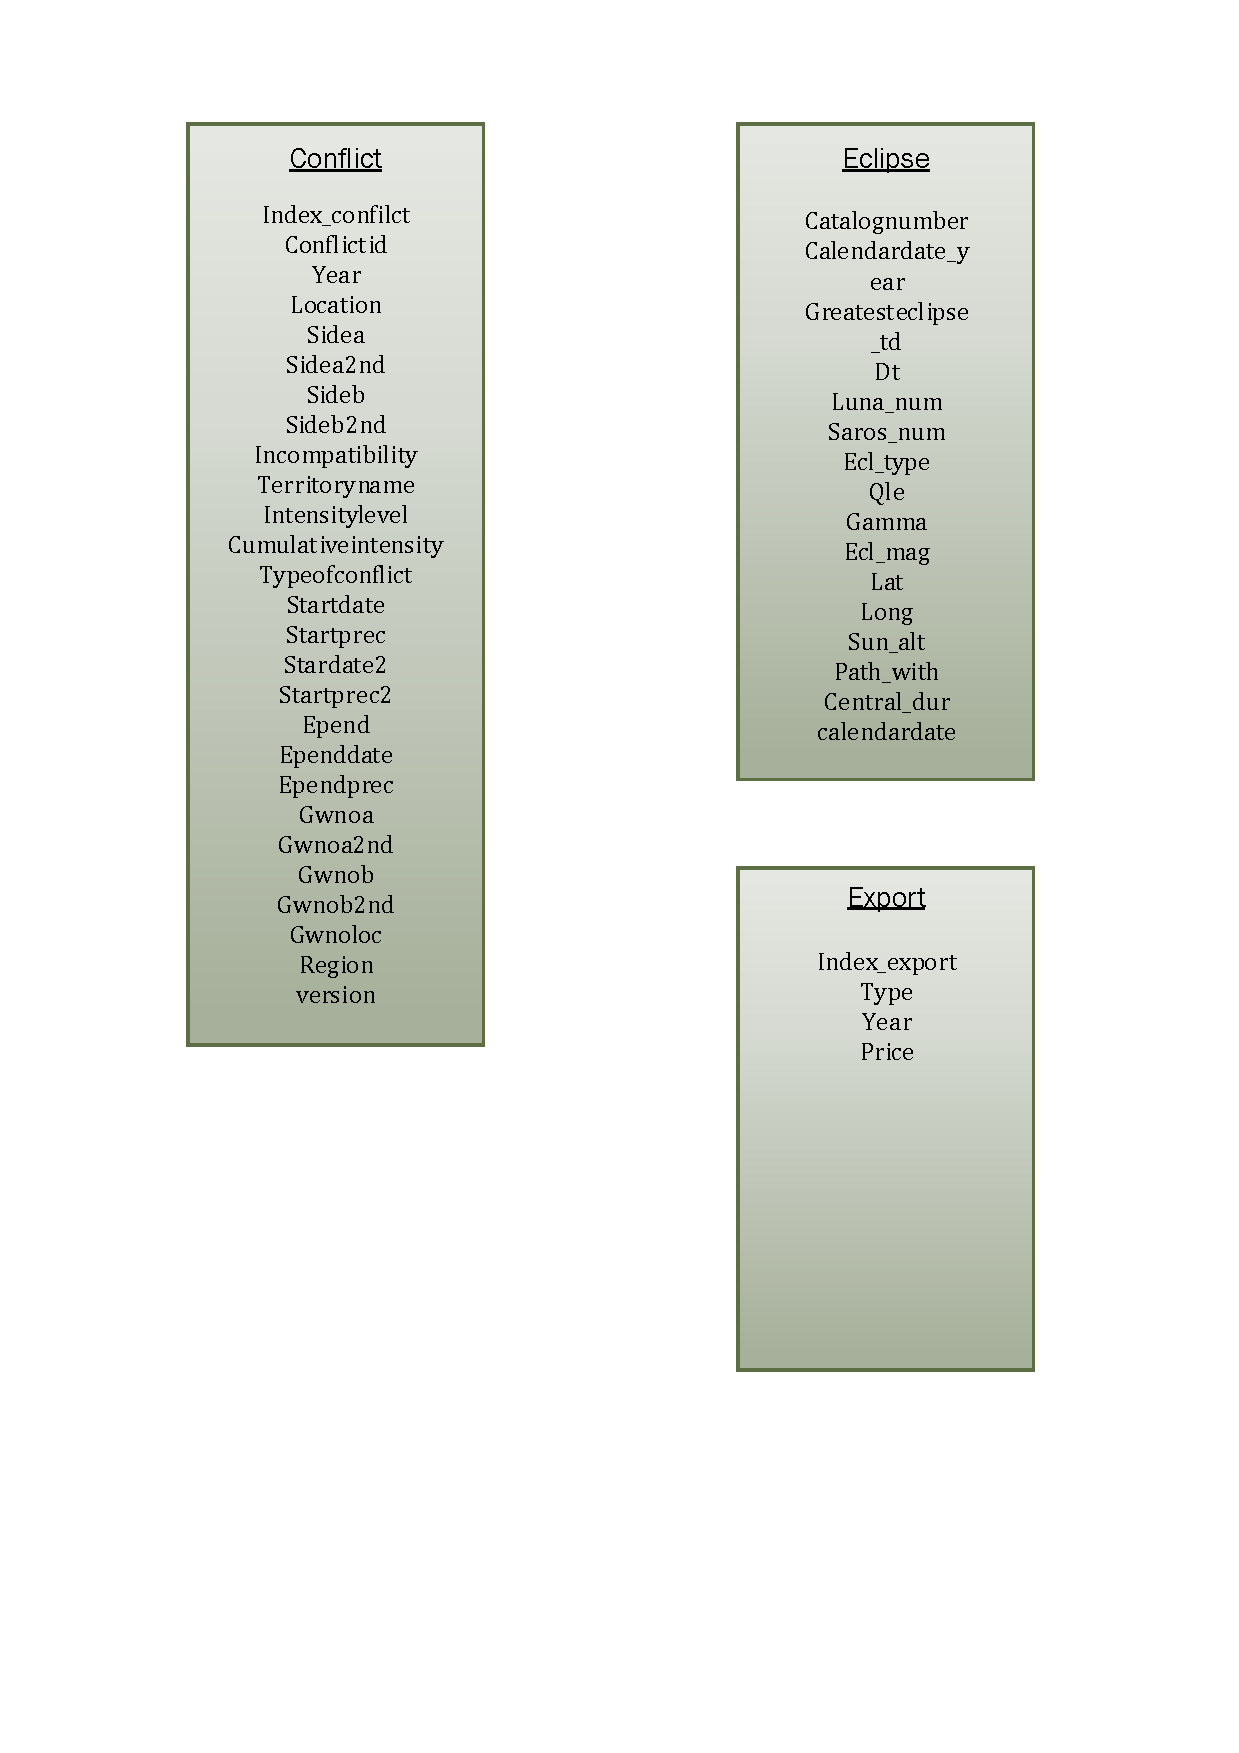
\includegraphics[width = 18cm]{dataSchema.pdf}
	\caption{Database schema \label{fig:dataschema}}
\end{figure} 
%
\begin{figure}
	\centering 
	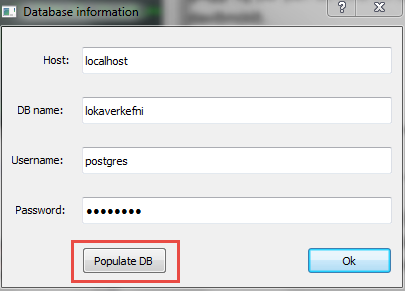
\includegraphics[width = 8cm]{logInScreen.png}
	\caption{Innskráningar glugginn \label{fig:logScreen}}
\end{figure} 

\begin{figure}
	\centering 
	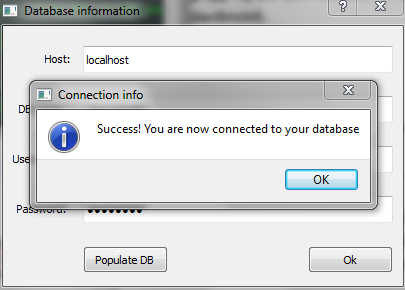
\includegraphics[width = 8cm]{logInSuccess.png}
	\caption{Staðfestingar gluggi á innskráningu \label{fig:logsucces}}
\end{figure} 

\begin{figure}
	\centering 
	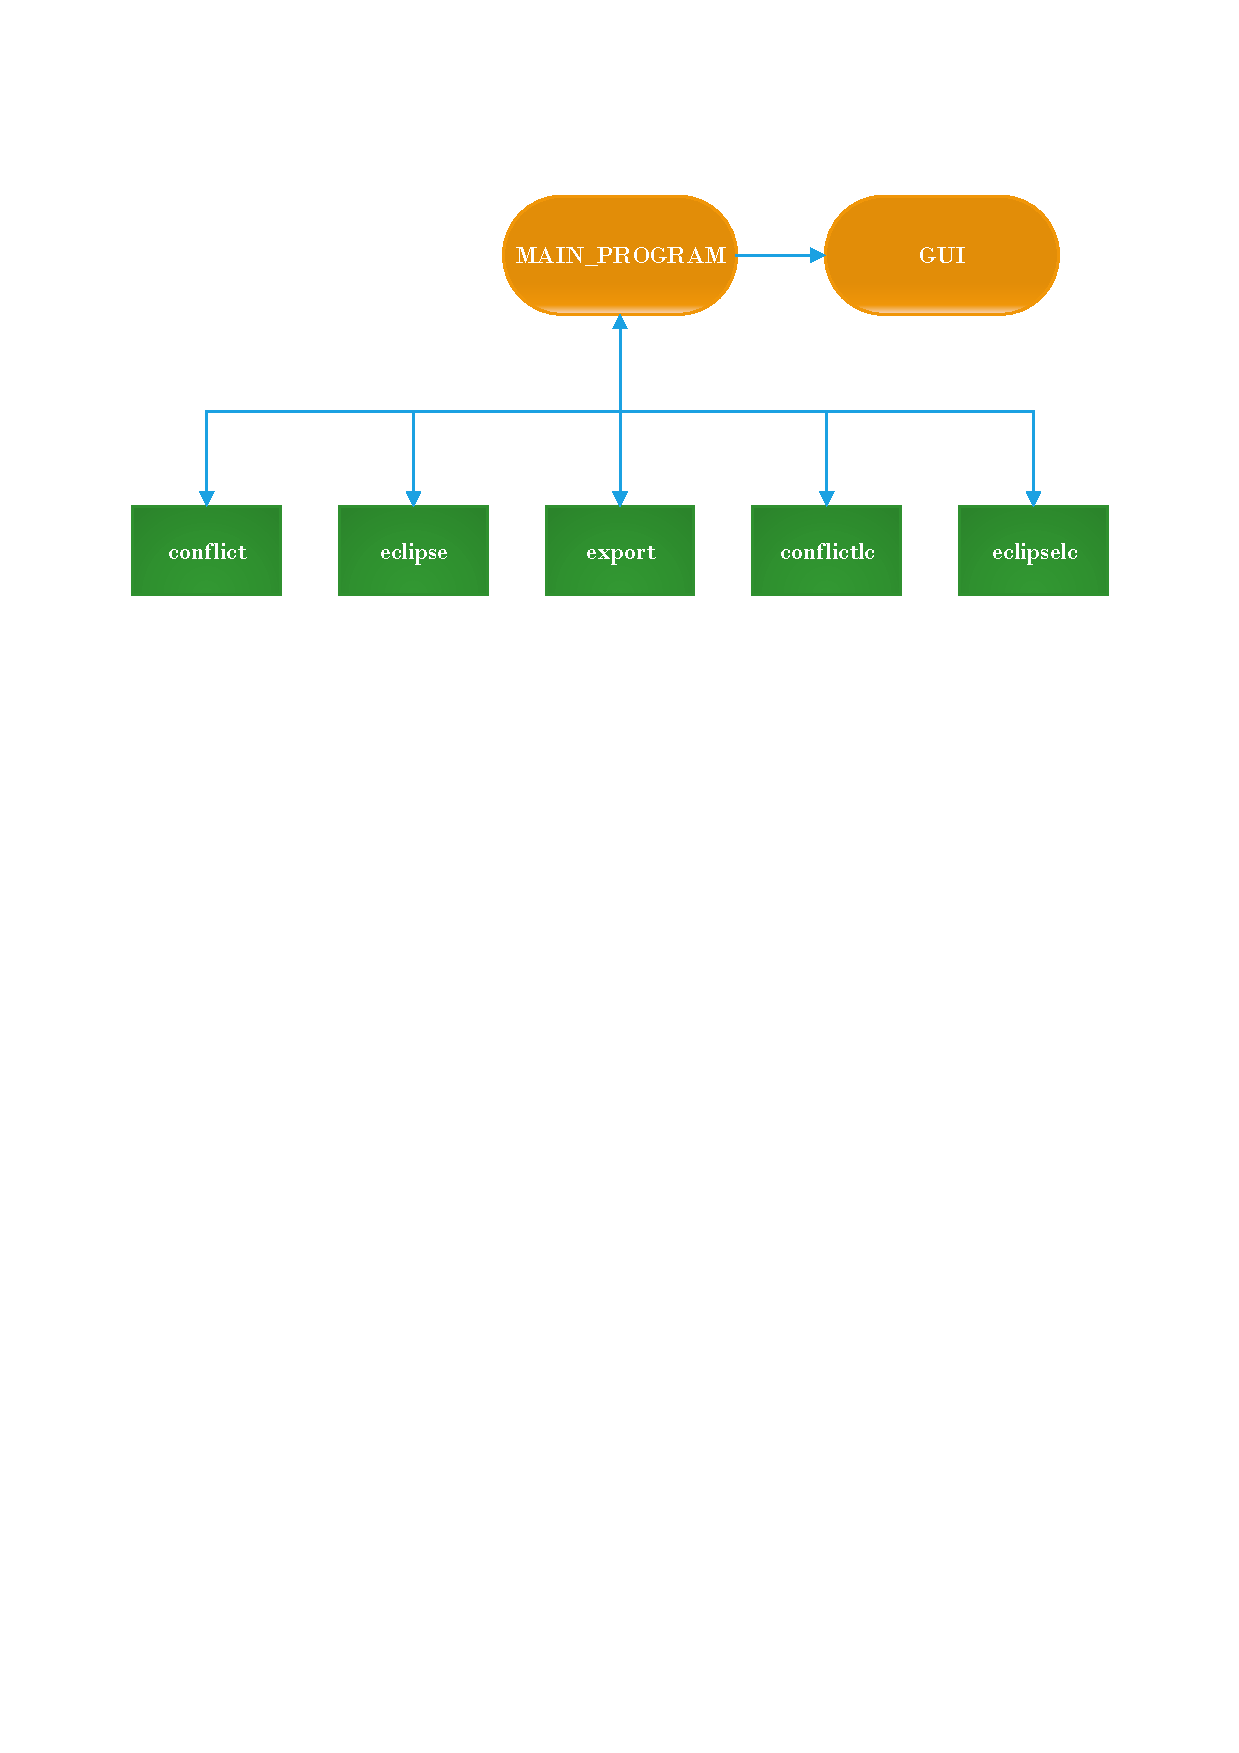
\includegraphics[width = 14cm,trim = 0pt 11cm 0pt 1cm, clip]{ufo.pdf}
	\caption{Staðfestingar gluggi á innskráningu \label{fig:diagram}}
\end{figure}

\begin{figure}[t]
	\centering 
	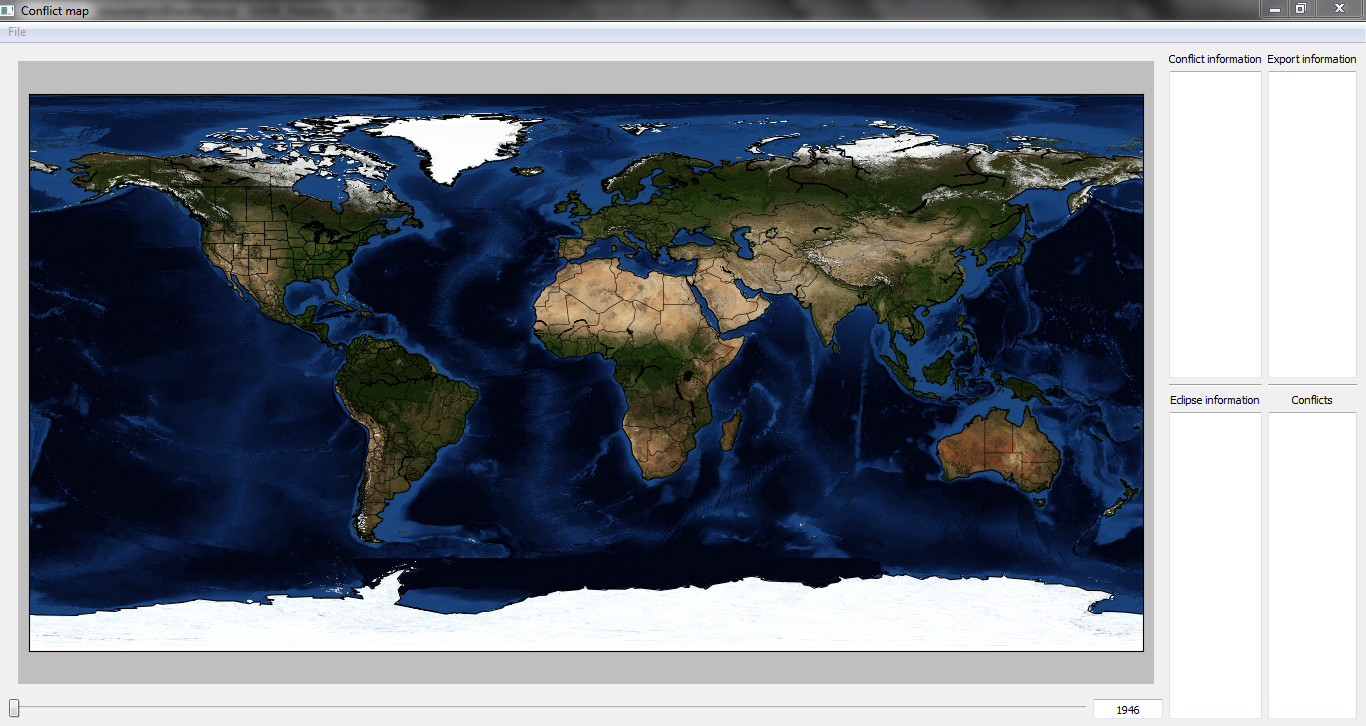
\includegraphics[width = 18cm]{openScreen.png}
	\caption{Aðalgluggi \label{fig:openScreen}}
\end{figure} 

\clearpage

\printbibliography

\end{document} % this tells the compiler that we are done

% These are variables for the editor Emacs
%%% Local Variables: 
%%% TeX-command-BibTeX: biber
%%% mode: latex
%%% TeX-master: t
%%% End:
